% This file was converted to LaTeX by Writer2LaTeX ver. 1.4
% see http://writer2latex.sourceforge.net for more info
\documentclass[twoside,a4paper]{article}
\usepackage[utf8]{inputenc}
\usepackage[T2A,T1]{fontenc}
\usepackage[russian,english]{babel}
\usepackage{amsmath}
\usepackage{amssymb,amsfonts,textcomp}
\usepackage{color}
\usepackage{array}
\usepackage{supertabular}
\usepackage{hhline}
\usepackage{hyperref}
\hypersetup{pdftex, colorlinks=true, linkcolor=blue, citecolor=blue, filecolor=blue, urlcolor=blue, pdftitle=EQUIPMENT}
\usepackage[pdftex]{graphicx}
% footnotes configuration
\makeatletter
\renewcommand\thefootnote{\arabic{footnote}}
\makeatother
% Outline numbering
\setcounter{secnumdepth}{0}
\makeatletter
\newcommand\arraybslash{\let\\\@arraycr}
\makeatother
% Page layout (geometry)
\setlength\voffset{-1in}
\setlength\hoffset{-1in}
\setlength\topmargin{0.3937in}
\setlength\oddsidemargin{0.7874in}
\setlength\evensidemargin{0.5909in}
\setlength\textheight{9.8016in}
\setlength\textwidth{6.8897996in}
\setlength\footskip{0.7484in}
\setlength\headheight{0.1972in}
\setlength\headsep{0.1583in}
% Footnote rule
\setlength{\skip\footins}{0.0469in}
\renewcommand\footnoterule{\vspace*{-0.0071in}\setlength\leftskip{0pt}\setlength\rightskip{0pt plus 1fil}\noindent\textcolor{black}{\rule{0.25\columnwidth}{0.0071in}}\vspace*{0.0398in}}
% Pages styles
\makeatletter
\newcommand\ps@Standard{
  \renewcommand\@oddhead{\textstylePageNumber{\hfill }}
  \renewcommand\@evenhead{}
  \renewcommand\@oddfoot{[Warning: Draw object ignored]}
  \renewcommand\@evenfoot{[Warning: Draw object ignored]}
  \renewcommand\thepage{\arabic{page}}
}
\makeatother
\pagestyle{Standard}
\setlength\tabcolsep{1mm}
\renewcommand\arraystretch{1.3}
\title{EQUIPMENT}
\begin{document}
\clearpage\setcounter{page}{1}\pagestyle{Standard}
\section[9. \textcyrillic{О}\textcyrillic{б}\textcyrillic{щ}\textcyrillic{и}\textcyrillic{е}
\textcyrillic{з}\textcyrillic{а}\textcyrillic{м}\textcyrillic{е}\textcyrillic{ч}\textcyrillic{а}\textcyrillic{н}\textcyrillic{и}\textcyrillic{я}
\textcyrillic{о}
\textcyrillic{к}\textcyrillic{и}\textcyrillic{т}\textcyrillic{а}\textcyrillic{й}\textcyrillic{с}\textcyrillic{к}\textcyrillic{о}\textcyrillic{й}
\textcyrillic{ф}\textcyrillic{и}\textcyrillic{л}\textcyrillic{о}\textcyrillic{с}\textcyrillic{о}\textcyrillic{ф}\textcyrillic{и}\textcyrillic{и}]{\foreignlanguage{russian}{9.
Общие замечания о китайской философии}}
\subsection[Север и Юг]{\selectlanguage{russian} Север и Юг}

\bigskip

\begin{flushleft}
\tablefirsthead{}
\tablehead{}
\tabletail{}
\tablelasttail{}
\begin{supertabular}{|m{0.52055985in}|m{0.6768598in}|m{1.2997599in}|m{1.6927599in}|m{1.6031599in}|}
\hline
{\selectlanguage{russian} Север }

{\selectlanguage{russian} (Хань)} &
{\selectlanguage{russian} 1 - 2 урожая в год} &
{\selectlanguage{russian} Начало {\textquotedbl}истории{\textquotedbl} – \foreignlanguage{english}{IV} тысячелетие до
н.э. } &
{\selectlanguage{russian} Просо, свиньи, собаки. Экономическое {\textquotedbl}равенство{\textquotedbl} и хватка.} &
{\selectlanguage{russian} Конфуцианство:\newline
этика, рационализм.}\\\hline
{\selectlanguage{russian} Юг}

{\selectlanguage{russian} (Чу)} &
{\selectlanguage{russian} 2 - 3 урожая в год} &
{\selectlanguage{russian} Начало {\textquotedbl}истории{\textquotedbl} – \foreignlanguage{english}{VIII} тысячелетие до
н.э. } &
{\selectlanguage{russian} Рис, свиньи, собаки, буйволы, куры. Экономическое {\textquotedbl}неравенство{\textquotedbl} и
спайка.} &
{\selectlanguage{russian} Даосизм: мифопоэтика\newline
(северная форма и южное содержание).}\\\hline
\end{supertabular}
\end{flushleft}
{\selectlanguage{russian}\itshape
В Китае нет религии и нет бога в нашем понимании. \ \ А во что же они верят?}

{\selectlanguage{russian}
С самого начала \textbf{философия в Китае} развивалась в двух направлениях — прагматическом и мистическом. }

{\selectlanguage{russian}
\textit{Прагматическое} \textit{направление} интересовалось жизнью в обществе, человеческими отношениями, моральными
ценностями и управлением. }

{\selectlanguage{russian}
\textit{Второе направление} полагало высшей целью философии возвышение над повседневной жизнью и достижение уровня
сознания мудреца\footnote{\foreignlanguage{russian}{\ Так называли идеал просветленного человека, достигшего
}\foreignlanguage{russian}{\textit{мистического единения}}\foreignlanguage{russian}{ с Вселенной.}}. Однако мирские
дела тоже беспокоят и волнуют мудреца. }

{\selectlanguage{russian}
Мудрец объединяет в себе взаимодополняющие интуитивную мудрость и практическое знание, созерцание и общественную
деятельность, которые традиционно ассоциируются в китайской культуре с образами мудреца и правителя. По словам
Чжуан-цзы, полностью реализовавшие себя личности {\textquotedbl}посредством своей неподвижности становятся мудрецами,
посредством своего движения — правителями{\textquotedbl}.}

{\selectlanguage{russian}
Все философские учения одного направления включали элементы другого направления.}

{\selectlanguage{russian}
В \foreignlanguage{english}{VI} веке до н.э. эти два направления китайской философии развились в две самостоятельные
философские школы — \textbf{конфуцианство} и \textbf{даосизм}. }

{\selectlanguage{russian}
\textbf{Конфуцианство} — философия общественного устройства, здравого смысла и практических знаний. Оно снабдило
китайское общество системой образования и строгими предписаниями общественного этикета, создало этическую основу для
традиционной китайской системы родственных отношений, обладавшей очень сложной структурой и ритуалами почитания
предков. }

{\selectlanguage{russian}
\textbf{Даосизм}, напротив, в первую очередь ценил созерцание природы и постижение ее \textit{пути} (= дао). Человек
счастлив, следуя естественному порядку, действуя спонтанно и доверяя своей \textit{интуиции}.}

{\selectlanguage{russian}
Два направления — две противоположные\footnote{\foreignlanguage{russian}{\ Для нас.}} стороны китайской философии, но в
Китае в них всегда видели две стороны единой природы человека, и поэтому они были взаимодополняющими. Давая образование
детям, обращались к конфуцианству, а к даосизму стремились взрослые люди, которые хотели восстановить и развить
утраченную спонтанность, умерщвленную условностями общественной жизни. В
\foreignlanguage{english}{XI}{}-\foreignlanguage{english}{XII} веках неоконфуцианцы предприняли успешную попытку
объединить в рамках своей школы конфуцианство, буддизм и даосизм. }

{\selectlanguage{russian}
Китайцы, подобно индийцам, считали, что существует высшая реальность, лежащая в основе многообразия вещей и явлений,
наблюдаемых нами, которая объединяет их:}

{\selectlanguage{russian}\itshape
{\textquotedbl}Есть три термина: {\textquotedbl}полное{\textquotedbl}, {\textquotedbl}всеохватывающее{\textquotedbl},
{\textquotedbl}целостное{\textquotedbl}. Они отличаются друг от друга, однако та реальность, которую они стремятся
отразить, одна и та же, — Единственное{\textquotedbl}.}

{\selectlanguage{russian}
\textbf{Китайский язык} совершенно не похож на знакомые нам европейские языки. {\textquotedbl}Слова{\textquotedbl} могут
выступать в нем в роли существительных, прилагательных или глаголов, не отличаясь при этом по формальным признакам
частей речи, а порядок {\textquotedbl}слов{\textquotedbl} определяется не столько грамматикой, сколько эмоциональным
содержанием предложения. Слово в классическом китайском языке вовсе не абстрактный знак, соответствующий четко
очерченному понятию, а символ, предназначенный вызывать в сознании нерасчлененный комплекс красочных картин и эмоций.
Текст стремится не столько сообщить некую цепочку интеллектуальных рассуждений, сколько поразить и удивить слушателя.
\textbf{Иероглиф} — не абстрактный знак, а органический образ, {\textquotedbl}гештальт{\textquotedbl}. Большая часть
образов теряется при переводе на европейские языки. Перевод одной фразы из {\textquotedbl}Дао-дэ цзин{\textquotedbl}
может передать лишь незначительную часть богатого комплекса идей, содержащегося в оригинале. Именно поэтому разные
переводы с одного и того же китайского оригинала на {\textquotedbl}наши языки{\textquotedbl} часто выглядят как
самостоятельные произведения. }

\begin{center}
\tablefirsthead{}
\tablehead{}
\tabletail{}
\tablelasttail{}
\begin{supertabular}{|m{2.49626in}|m{3.17816in}|}
\hline
\centering{\selectlanguage{russian}\bfseries Запад} &
\centering\arraybslash{\selectlanguage{russian}\bfseries Китай}\\\hline
{\selectlanguage{russian} Наука упорядочивает Хаос} &
{\selectlanguage{russian} В основе мира - порядок, основанный на \ этике}\\\hline
{\selectlanguage{russian} Мужики (Уран, Зевс) правят миром} &
{\selectlanguage{russian} В основе мира женское \textit{дао}}\\\hline
{\selectlanguage{russian} Бог пасет народы} &
{\selectlanguage{russian} Народ пасется, правитель {\textquotedbl}неподвижен{\textquotedbl}}\\\hline
{\selectlanguage{russian} Человек – субъект деятельности} &
{\selectlanguage{russian} Человек – объект деятельности}\\\hline
{\selectlanguage{russian} Власть ради выгоды} &
{\selectlanguage{russian} Власть ради власти}\\\hline
{\selectlanguage{russian} Наводить порядок!} &
{\selectlanguage{russian} Следовать порядку}\\\hline
{\selectlanguage{russian} Смена парадигм} &
{\selectlanguage{russian} Взаимопроникновение парадигм}\\\hline
{\selectlanguage{russian} Конфессия = комплекс ритуалов} &
{\selectlanguage{russian} Комплекс ритуалов = комплекс {\textquotedbl}конфессий{\textquotedbl}}\\\hline
\end{supertabular}
\end{center}
\section[10. Инь{}-ян]{\selectlanguage{russian} 10. Инь-ян}
{\selectlanguage{russian}
\textbf{Инь-ян} выражает универсальную концепцию дуализированности мира в бесконечном ряду бинарных (дихотомических)
оппозиций: темное и светлое, пассивное и активное, мягкое и твердое, внутреннее и внешнее, нижнее и верхнее, женское и
мужское, земное и небесное и т.д. }

{\selectlanguage{russian}\itshape
Этимологические корни \ \textbf{инь} \textup{и} \textbf{ян} – теневой и солнечный склоны холма. }

{\selectlanguage{russian}
В \foreignlanguage{english}{V}–\foreignlanguage{english}{III} веках до н.э. \textit{инь} и \textit{ян} впервые
представлены как две ипостаси эфира — соответственно «земная» и «небесная», нарушение порядка взаимодействия которых
приводит к стихийным бедствиям и смутам. В \foreignlanguage{english}{IV}–\foreignlanguage{english}{III} веках до н.э. с
взаимодействием \textit{инь-ян} сопряжены смена времен года, дня и ночи. В~\foreignlanguage{english}{IV} в. до н.э.
\textit{инь-ян} связаны с категориями Дао-дэ цзина «покой» и «движение». \textit{Инь-ян} знаменует собой первый шаг от
недифференцированного единства первозданного эфира к многообразию всей «тьмы вещей». Связь \textit{инь-ян} и
\textit{дао} такова: «одно \textbf{инь}, одно \textbf{ян} – это и есть \textbf{дао}». }

\begin{flushleft}
\tablefirsthead{}
\tablehead{}
\tabletail{}
\tablelasttail{}
\begin{supertabular}{m{2.87126in}m{4.01086in}}
\centering  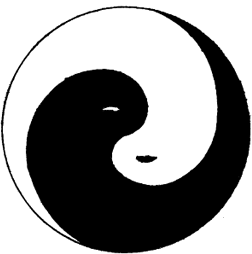
\includegraphics[width=1.0209in,height=1.0264in]{a913-img001.png}  &
{\selectlanguage{russian} Прототипы этого S-образного символа \ обнаруживаются в древнейших произведениях китайской
материальной культуры, восходящих к неолиту. Нильс Бор признал в нем наилучшую иллюстрацию для своего принципа
дополнительности. }\\
\end{supertabular}
\end{flushleft}
{\selectlanguage{russian}
\textit{Инь} и \textit{ян} в свою очередь делятся на \textit{инь-ян} — и так без конца. Эта концепция универсального
дуализма вошла практически во все философские и научные построения.}

{\selectlanguage{russian}
Действие \textit{инь-ян} было распространено на общественные и семейные отношения: «Все дурное исчерпывается в
\textit{инь}, все доброе — в \textit{ян}; в \textit{ян} — высокое начало, в \textit{инь} — низкое». В средние века
рождение \textit{инь-ян} в динамике «движения» и «покоя» определилось как программа упорядоченного развития мира.
\textbf{Взаимопроникновение} \textbf{инь-ян} обеспечивает (относительную) устойчивость всех субстанциальных
образований. \textit{Инь} и \textit{ян} \ находятся друг в друге, а не противоположны друг другу. Каждое из этих начал
содержит в себе в потенции другое (см. рисунок): так устроено все сущее в мире.}

{\selectlanguage{russian}
Ныне концепция \textit{инь-ян} продолжает играть важную роль в теории китайской медицины.}

{\selectlanguage{russian}
В западных ценностных ориентирах преобладают \textit{ян}–ценности, выраженные в рациональных, мужественных и агрессивных
настроениях. Типичный пример \textit{ян}–ориентации — {\textquotedbl}наши{\textquotedbl} ученые.}

{\selectlanguage{russian}
Для перехода к динамическому равновесию Западу нужно усвоить восточные \textit{инь}–принципы и научиться воспринимать
мир в его целостности, в согласии со всем мирозданием.}


\bigskip

\begin{flushleft}
\tablefirsthead{}
\tablehead{}
\tabletail{}
\tablelasttail{}
\begin{supertabular}{m{3.4406598in}m{3.44136in}}
{\centering\selectlanguage{english} \foreignlanguage{russian}{\ \ \ \ Но выше просится душа,}\par}

{\centering\selectlanguage{russian} И что, ее всегда чаруя,\par}

{\centering\selectlanguage{russian} Зовет и манит вдалеке,\par}

{\centering\selectlanguage{english} \foreignlanguage{russian}{\ \ \ \ О том поведать не могу я}\par}

{\centering\selectlanguage{russian} На ежедневном языке.\par}

{\selectlanguage{russian} \textit{\ \ \ \ \ \ А.К. Толстой – И.С. Аксакову}} &
{\centering\selectlanguage{english} \foreignlanguage{russian}{\ \ Как сердцу высказать себя?}\par}

{\centering\selectlanguage{russian} Другому, как понять тебя?\par}

{\centering\selectlanguage{english} \foreignlanguage{russian}{\ \ \ \ \ \ \ \ Поймет ли он, чем ты живешь?}\par}

{\centering\selectlanguage{english} \foreignlanguage{russian}{\ \ \ \ Мысль изреченная есть ложь.}\par}

~

{\selectlanguage{russian} \textit{\ \ \ \ \ \ \ \  \ \ \ Ф.И. Тютчев \ }}\\
\end{supertabular}
\end{flushleft}
\section[11. Даосизм]{\selectlanguage{russian} 11. Даосизм}
{\selectlanguage{russian}
Даосизм \ сформировался ко \foreignlanguage{english}{II} веку до н.э. Его истоки — в южных шаманских верованиях. Это
учение впервые представлено в \textit{{\textquotedbl}Дао-дэ цзин{\textquotedbl}. }Даосизм как система (в европейском
понимании) сформирован на Юге Чжан Дао-линем\textit{ }как синтез учения Лао\nobreakdash-цзы и\textit{ }доктрины
\textit{инь-ян. }}

{\selectlanguage{russian}
Чжан Дао-лин\textit{ }основал {\textquotedbl}Путь Небесных наставников{\textquotedbl}, получив от обожествленного
Лао-цзы откровение и одновременно право быть его наместником на земле. Титул {\textquotedbl} Небесного
наставника{\textquotedbl} передается в роду Чжан по наследству до настоящего времени. }

{\selectlanguage{russian}
Южный даосизм элитарен, а северные направления даосизма тяготели к активному воздействию на коллективы верующих
{\textquotedbl}из народа{\textquotedbl}. В \foreignlanguage{english}{VII} - \foreignlanguage{english}{VIII} веках под
влиянием буддизма\textit{ }возникают монашество и монастыри. }

{\selectlanguage{russian}
Разные направления имели равный статус, на их основе возникали секты, с которыми ортодоксы вели такую же непримиримую
борьбу, как и конфуцианство. {\textquotedbl}Ереси{\textquotedbl} часто становились базой тайных обществ
(\textit{Тайпин} \textit{дао} — {\textquotedbl}Путь Великого равенства{\textquotedbl}, \textit{Байлянь цзяо }—\textit{
}{\textquotedbl}Учение Белого лотоса{\textquotedbl} и др.) и крестьянских выступлений. Восстание {\textquotedbl}Желтых
повязок{\textquotedbl} в 184 г. сокрушило империю Хань. }

{\selectlanguage{russian}
Танские императоры (618 —917 гг.) считали себя потомками Лао-цзы.}

{\selectlanguage{russian}
Конфуциански образованная интеллектуальная элита проявляла интерес к философии даосизма, особенно после падения Хань и
дискредитации ее официальной идеологии — конфуцианства. }

{\selectlanguage{russian}
Даосизм предоставил буддизму аппарат для перевода его понятий в привычные для китайцев формы. Даосизм воспринял
буддийские методы медитации и организационные структуры. Иные считали Будду сыном Лао-цзы, иные считали их одним и тем
же Учителем. }

{\selectlanguage{russian}
В эпоху династии Сунн (960 — 1124 гг.) создан текст {\textquotedbl}Даосского канона{\textquotedbl}.}

{\selectlanguage{russian}
В \foreignlanguage{english}{XII} веке появляется и вплоть до настоящего времени является ведущим направлением в даосизме
школа {\textquotedbl}Учение Совершенной истины{\textquotedbl}. }

{\selectlanguage{russian}
Даосизм не имел успеха в Корее и в Японии, но даосские тексты вошли в японскую культуру. }

\subsubsection{Учение Дао}
{\selectlanguage{russian}
Основные категории: \textit{Дао, дэ, ци.}}

{\selectlanguage{russian}
\textbf{Дао}: {\textquotedbl}Путь{\textquotedbl}, {\textquotedbl}подход{\textquotedbl},
{\textquotedbl}функция{\textquotedbl}, {\textquotedbl}метод{\textquotedbl},
{\textquotedbl}закономерность{\textquotedbl}, {\textquotedbl}принцип{\textquotedbl},
{\textquotedbl}класс{\textquotedbl}, {\textquotedbl}учение{\textquotedbl}, {\textquotedbl}теория{\textquotedbl},
{\textquotedbl}правда{\textquotedbl}, {\textquotedbl}мораль{\textquotedbl}, {\textquotedbl}абсолют{\textquotedbl}.
Европейскими эквивалентами \textit{дао} часто признается Логос = разум как доминанта Мира, противостоящая хаосу и
порождающая гармонию. }

{\selectlanguage{russian}\itshape
Иероглиф Дао входит в обозначение даосизма (дао цзя) и неоконфуцианства (дао сюэ). }

{\selectlanguage{russian}
\textit{\ }В различных системах \textit{дао} определялось по-разному, поэтому \textit{Хань Юй
}(\foreignlanguage{english}{VIII}{}-\foreignlanguage{english}{IX} вв. н.э.) назвал его {\textquotedbl}пустой
позицией{\textquotedbl}, не имеющей точно фиксированного смысла. В узком смысле {\textquotedbl}небесное
дао{\textquotedbl} означало ход времени или движение звезд с запада на восток в противоположность движению солнца с
востока на запад.}

{\selectlanguage{russian}
Главное проявление \textit{дао} - {\textquotedbl}перемены{\textquotedbl}, трансформации по принципу {\textquotedbl}то
\textit{инь} — то \textit{ян}{\textquotedbl} в неизменном порядке изменчивости.}

{\selectlanguage{russian}\itshape
Колесо движется, потому что ось неподвижна.}

{\selectlanguage{russian}\itshape
Покой есть главное в движении (поэтому оно не переходит в хаос).}

{\selectlanguage{russian}
\textbf{Дэ}: {\textquotedbl}Добродетель{\textquotedbl}, {\textquotedbl}благодать{\textquotedbl}
({\textquotedbl}качество{\textquotedbl}, {\textquotedbl}дарование{\textquotedbl},
{\textquotedbl}достоинство{\textquotedbl}, {\textquotedbl}достояние{\textquotedbl},
{\textquotedbl}доблесть{\textquotedbl}, {\textquotedbl}моральная сила{\textquotedbl},
{\textquotedbl}закономерность{\textquotedbl}). В самом общем смысле — качество, обусловливающее наилучший способ
существования существа или вещи. \textit{Дэ} относительно (в отличие от всеобщего и потому абсолютного \textit{дао}),
поэтому {\textquotedbl}благодать{\textquotedbl} для одних может негативно оцениваться другими.
{\textquotedbl}Благодатью{\textquotedbl} следует отвечать на {\textquotedbl}благодать{\textquotedbl}, а не на вражду.
Благодать {\textquotedbl}благородного мужа{\textquotedbl} доминирует над благодатью {\textquotedbl}ничтожного
человека{\textquotedbl}, как ветер над травой. Идеальна гармония между \textit{дэ} правителя и подданных. }

{\selectlanguage{russian}\itshape
{\textquotedbl}Знать, что тут ничего не поделаешь, и спокойно принимать это как предопределение — есть предел
благодати{\textquotedbl}. }

{\selectlanguage{russian}
Европейцы воспринимают \textit{дэ} как моральный императив (по Канту).}

{\selectlanguage{russian}
\textbf{Ци}: {\textquotedbl}Орудие{\textquotedbl}, {\textquotedbl}явление{\textquotedbl},
{\textquotedbl}способность{\textquotedbl}. \textit{Ци — космическая энергия. \ Дао} противопоставляется \textit{ци}. В
качестве {\textquotedbl}отсутствия/небытия{\textquotedbl} \textit{дао} определяет \textit{ци} как сосуд,
{\textquotedbl}орудие{\textquotedbl} \textit{дао}. }

{\selectlanguage{russian}
\textbf{Небесное дао} утверждается силами \textit{инь} и \textit{ян, }\textbf{земное} —
{\textquotedbl}мягкостью{\textquotedbl} и {\textquotedbl}твердостью{\textquotedbl}, \textbf{человеческое} —
{\textquotedbl}гуманностью{\textquotedbl} и {\textquotedbl}долгом/справедливостью{\textquotedbl}. }

{\selectlanguage{russian}\itshape
Четыре сферы реализации дао: в речах, поступках, изготовлении орудий, гаданиях.}

{\selectlanguage{russian}
Даосизм оппозиционен конфуцианской теории, \ делая упор на небесную, а не человеческую ипостась \textit{дао}.
Конфуцианцы исходили из словесно-понятийной выразимости и даже самовыразимости \textit{дао}, даосизм заявил о
словесно-понятийной невыразимости и непознаваемости \textit{дао}. {\textquotedbl}Завершение, при котором неведомо,
почему так, называется \textit{дао}{\textquotedbl}. }

{\selectlanguage{russian}
\textbf{Современная трактовка}. \textit{Дао }рождает одно — \textit{ци}; из \textit{ци} состоит все в мире. Одно
\textit{ци} рождает два \ — \textit{ян-ци} и \textit{инь-ци} (мужское и женское). Два рождают три — \textit{Небо},
\textit{Землю} и \textit{Человека}. }

{\selectlanguage{russian}\itshape
Даосизм не для всех был {\textquotedbl}только теорией{\textquotedbl}: император Цинь Ши-хуанди (221 г. до н.э.) снаряжал
экспедиции к бессмертным. }


\bigskip

\section[12. Конфуцианство]{\selectlanguage{russian} 12. Конфуцианство}
{\selectlanguage{russian}
\textbf{Конфуций} (Кун-цзы) — около 551-479 до н. э., современник Будды. Основные взгляды Конфуция изложены его
учениками (а не им самим) в книге {\textquotedbl}Лунь юй{\textquotedbl} ({\textquotedbl}Беседы и
суждения{\textquotedbl}).}

\subsubsection[\ Жизнь]{\ Жизнь}
{\selectlanguage{russian}
В молодости работал управляющим складами и надсмотрщиком над стадами, затем получил должность помощника при совершении
жертвоприношений в главной кумирне царства Лу. В 50 лет впервые оказался на государственной службе, но пост первого
советника покинул почти сразу же: к его советам никто не прислушался. Следующие 13 лет он посещал властителей Китая,
стремясь склонить их к принятию своего этико-политического учения, — успеха не имел. В конце концов, Конфуций целиком
посвятил себя педагогической деятельности. Конфуций считается первым частным учителем в Китае. Его известность как
знатока книг, ритуала и музыки привлекла к нему множество учеников, составивших собрание его суждений и диалогов —
{\textquotedbl}Лунь юй{\textquotedbl}. }

\subsubsection{Учение }
{\selectlanguage{russian}
Подчеркивая свою приверженность традиции, Конфуций говорил: {\textquotedbl}Я передаю, но не создаю; я верю в древность и
люблю ее{\textquotedbl}. Золотым веком Конфуций считал первые годы правления династии Чжоу (1027-256 гг. до н.э.)
Напротив, современность представлялась ему царством хаоса. Нескончаемые междоусобные войны, все усиливающаяся смута
привели Конфуция к выводу о необходимости для Китая новой моральной философии, которая опиралась бы на представление об
изначальном добре, заложенном в каждом человеке. Прототип нормального общественного устройства Конфуций видел в добрых
семейных отношениях, когда старшие любят младших и заботятся о них (\textit{жэнь}, принцип
{\textquotedbl}человечности{\textquotedbl}), а младшие, в свою очередь, отвечают любовью и преданностью (\textit{и},
принцип {\textquotedbl}справедливости{\textquotedbl}). Особенно подчеркивалась важность исполнения сыновнего долга
(\textit{сяо} — {\textquotedbl}сыновняя почтительность{\textquotedbl}). Мудрый правитель должен управлять с помощью
воспитания у подданных чувства благоговения перед {\textquotedbl}ритуалом{\textquotedbl}, то есть моральным законом,
прибегая к насилию только как к последнему средству. Отношения в государстве во всем должны быть подобны отношениям в
хорошей семье: {\textquotedbl}Правитель должен быть правителем, подданный — подданным, отец — отцом, сын —
сыном{\textquotedbl}. Конфуций поощрял традиционный культ предков как средство сохранения верности родителям, роду и
государству, в состав которого тем самым бы входили все живые и все умершие. Долгом всякого {\textquotedbl}благородного
мужа{\textquotedbl} Конфуций считал бесстрашное и нелицеприятное обличение любых злоупотреблений.}

{\selectlanguage{russian}
Конфуций конкретизировал \textit{дао} в наборах понятий: {\textquotedbl}сыновняя почтительность{\textquotedbl} и
{\textquotedbl}братская любовь{\textquotedbl}, {\textquotedbl}верность{\textquotedbl} и
{\textquotedbl}великодушие{\textquotedbl}, {\textquotedbl}гуманность{\textquotedbl} (\textit{жэнь}),
{\textquotedbl}знание{\textquotedbl} и {\textquotedbl}мужество{\textquotedbl}. \ \ В силу различия носителей различны и
их \textit{дао}: прямое и кривое, большое и малое, присущее {\textquotedbl}благородному мужу{\textquotedbl} и
{\textquotedbl}ничтожному человеку{\textquotedbl}. Соответственно разнятся и \textit{дэ}. }

{\selectlanguage{russian}
При отсутствии \textit{дао} в Поднебесной следует {\textquotedbl}скрываться{\textquotedbl}, отказываться от службы,
посвящать себя только семье. }

\subsubsection[Культ Конфуция \ и \ конфуцианство ]{Культ Конфуция \ и \ конфуцианство }
{\selectlanguage{english}
\foreignlanguage{russian}{Конфуций не был основателем религии; на вопрос одного из учеников о загробном мире ответил:
{\textquotedbl}Не научившись [честно] служить людям, можно ли [достойно] служить духам?{\textquotedbl}. Однако в его
честь были воздвигнуты храмы, стал складываться религиозный по форме культ первоучителя человечества. Конфуцианство
приобрело в Китае статус официального учения, благодаря системе экзаменов государственные должности могли занимать
только ученые конфуцианцы (конфуцианское учение понималось как {\textquotedbl}наука{\textquotedbl} вообще, а
конфуцианцы — как {\textquotedbl}}\foreignlanguage{russian}{\textit{жу}}\foreignlanguage{russian}{{\textquotedbl}, т.
е. {\textquotedbl}ученые{\textquotedbl}, {\textquotedbl}образованные{\textquotedbl}). Уже первый император ханьской
династии Гао-цзу посетил могилу Конфуция на его родине и принес в жертву быка. Через 50 лет был воздвигнут храм в честь
Конфуция. В 267~г. императорским указом предписано приносить в столице и на родине Конфуция четырежды в год в жертву
овцу, свинью и быка. В 555~г. предписано сооружение в каждом городе, где есть представитель власти, храма в честь
Конфуция. В~начале ХХ века род Конфуция насчитывал 20-30 тыс. членов, он существует и ныне. Старший потомок Конфуция по
прямой линии носит наследственный княжеский титул, при императорах он должен был посвящать себя уходу за могилой
великого предка. }}

\subsubsection{Практика}
{\selectlanguage{russian}
Земледелец — раб земли — нуждается в защите. На земле растут не только злаки, но и государство с городами, армиями и,
конечно, властителями (на них возложено разделение пищи и труда). С \foreignlanguage{english}{VII} по
\foreignlanguage{english}{IV} век до н.э. \textit{легисты} создали 20-уровневую вертикаль власти: от пятерки
домохозяйств, связанных круговой порукой перед следующим уровнем власти, до \textit{вана}, имеющего мандат от Неба как
нравственно совершенный человек.\footnote{\foreignlanguage{russian}{\ Совсем как у нас!}} Государство = большая семья,
поэтому цель нравственного развития — государственная служба. Продвижение по службе обеспечивала государственная
система образования и экзаменов.\footnote{\foreignlanguage{russian}{\ Существовала до 1905 года. Представьте традицию
такого возраста у нас. Представили?..}} Сдавший экзамен самой первой ступени (уездный \textit{сю цай}: знал около 3
тысяч иероглифов, мог написать поэму в 60 знаков о событии в древности) получал освобождение от налогов и от телесных
наказаний (нам бы вот так!). Уважаемый \textit{сю цай} мог сдавать следующий экзамен даже в старости: экзамен — дело
серьезное. На высоких ступенях требовалось иметь не менее трех поколений предков, сдавших экзамены. Конкурсные экзамены
высшей ступени проводились один раз в 2-3 года в присутствии \textit{вана}. Запад заимствовал экзамены у Китая.}

{\selectlanguage{russian}\itshape
Процедура формирования китайской элиты вряд ли поддается пониманию нашей элитой.}

{\selectlanguage{russian}\itshape
Чиновник получал отставку на 2 года для пребывания в трауре по умершим родителям.}

{\selectlanguage{russian}\itshape
\textbf{Цинь Ши-хуанди }однажды\textbf{ }навел порядок, используя властную вертикаль: зарыл живьем 460 конфуцианских
мудрецов и сжег все неугодные ему книги.}

\subsubsection{Мораль}
{\selectlanguage{russian}
{\textquotedbl}Гармония{\textquotedbl} (\textit{хэ}) составляет всепроникающее Дао Поднебесной, выраженное в пяти видах
отношений: между правителем и подданным, отцом и детьми, мужем и женой, старшими и младшими братьями, друзьями\textit{.
}Осуществляется \textit{хэ} посредством {\textquotedbl}знания{\textquotedbl}, {\textquotedbl}гуманности{\textquotedbl}
и {\textquotedbl}мужества{\textquotedbl} — троякой {\textquotedbl}великой благодати{\textquotedbl} \textit{(да дэ)
}Поднебесной. }

{\selectlanguage{russian}
Благородный человек действует по долгу, \textit{сяо жэнь} – по выгоде.}

{\selectlanguage{russian}
На обыденном уровне познание и осуществление \textit{дао} доступно даже глупым и никчемным \textit{сяо жэнь}, но в своем
предельном выражении оно содержит нечто непознаваемое и неосуществимое даже для
{\textquotedbl}совершенномудрых{\textquotedbl}. }

\subsubsection{Да тун - великое единение }
{\selectlanguage{russian}
«Великое единение» — одна из основных утопических социально-политических концепций конфуцианства. Главный компонент
бинома \textit{да тун} – понятие «\textit{тун}» («единение, объединение, совместимость, тождественность») имеет разные
значения. Например, в Чжоу-ли (\foreignlanguage{english}{V}–\foreignlanguage{english}{II} вв. до н.э.) — объединение из
10 тысяч территориальных единиц, «колодцев»; в Мо-цзы (\foreignlanguage{english}{V}–\foreignlanguage{english}{III} вв.
до н.э.) \textit{тун} определяется как «повторенность», «совместимость», «родственность». \textit{Да тун} впервые
прозвучало в Шу~цзине (\foreignlanguage{english}{VIII}–\foreignlanguage{english}{V} вв. до н.э.) как обозначение
результата разделения земли древним «совершенномудрым» правителем Юем на девять областей и образования
социально-политически, экономически и культурно иерархизированного множества территорий. В другом месте Шу~цзина
\textit{да тун} подразумевает такое положение в обществе, когда все инстанции, влияющие на принятие важного
государственного решения, единодушны. Перечисление этих инстанций (государь, оракулы, сановники, служилые люди, народ)
предполагает четкую социальную иерархию. }

{\selectlanguage{russian}
Собственно концепция \textit{да тун} впервые была представлена Конфуцием в описании двух состояний общества: идеальное —
\textit{да тун} и приемлемое — \textit{сяо кан} («малое процветание»). Определение сущности \textit{да тун} обычно
принято толковать примерно следующим образом: «Когда действовало Великое \textit{дао} (когда шли по Великому пути),
Поднебесная принадлежала всем (была общей). Ныне, когда Великое \textit{дао} уже скрылось, Поднебесная принадлежит
семьям». }

{\selectlanguage{russian}
\textit{Да тун} означает такое состояние Поднебесной, при котором все в ней гармонизировано как в здоровом едином
организме с естественной ненарушенной иерархией органов и функций. }

{\selectlanguage{russian}\itshape
Император подобен \ неподвижной Полярной звезде, ненасильственно управляющей движением всех звезд.}

\subsubsection{}
\subsubsection{{\textquotedbl}Вечное{\textquotedbl} учение}
{\selectlanguage{russian}
Две целостные и противоположные друг другу (ортодоксальная и неортодоксальная) интерпретации конфуцианства предложили
Мэн-цзы и Сюнь-цзы в IV - III веках до н.э; в первой – человек изначально добр; во второй — человек изначально зол, от
рождения стремится к выгоде и плотским наслаждениям. Мэн-цзы исследовал мораль и психологию (предложил теорию
{\textquotedbl}гуманного управления{\textquotedbl} с правом подданных свергать порочного государя), а Сюнь-цзы —
социальную и гносеопраксиологическую стороны человеческого существования (сформулировал задачу идеального государя –
{\textquotedbl}завоевание{\textquotedbl} своего народа). В эпоху Хань (III в. до н.э. — III в. н.э.) на этих основах
было создано {\textquotedbl}ханьское конфуцианство{\textquotedbl}. Возникшее в XI в. неоконфуцианство в XIV веке
получило официальное признание и стало основой понимания конфуцианской классики в системе государственных экзаменов
вплоть до 1912 года, доминировало в Корее, Японии, Вьетнаме (в Китае – до 1949 г.); ныне – на Тайване и в Сингапуре. }

{\selectlanguage{russian}
Официальное неоконфуцианство = космология + мораль + духовное совершенство. }

{\selectlanguage{russian}
Человек = человеческое сознание + небесное сознание = желания + чистота духа. }

{\selectlanguage{russian}
Знания и сознательность, расширяясь, устраняют (низменное) человеческое сознание. }

\subsection[Синтез учений]{\selectlanguage{russian} Синтез учений}
{\selectlanguage{russian}
Идеи даосизма активно использовались мыслителями направления \textbf{\textit{сюань сюэ.}}}

{\selectlanguage{russian}
\textit{Сюань сюэ} — «учение о таинственном», «учение о сокровенном» — течение
\foreignlanguage{english}{III}–\foreignlanguage{english}{IV} веков, своеобразный синтез даосизма, конфуцианства и даже
буддийской метафизики. }

{\selectlanguage{russian}
Первоначально учение имело форму комментариев к конфуцианской и даосской классике: {\textquotedbl}опираясь на Лао-цзы,
проникать в конфуцианство{\textquotedbl}. Категория «\textit{сюань}» («тайна, таинственное, сокровенное, непостижимое»)
восходит к первому параграфу Дао-дэ цзина, в котором она означает сверхъестественное «единение» (\textit{тун})
«отсутствия/небытия» и «наличия/бытия». В сфере небесного — это таинственное (\textit{сюань}), в сфере человеческого —
это \textit{дао}, в сфере земного — это превращение (\textit{хуа}). Ян Сюн (53 г. до н.э. – 18 г. н.э.) посвятил
категории «\textit{сюань}» универсальную теорию мировых процессов, в которой трактует \textit{дао} — «пустое по форме и
определяющее путь (\textit{дао}) вещей» — в качестве ипостаси «тайны», понимаемой как «предел деятельного проявления».
}

{\selectlanguage{russian}
В зависимости от признания всепроникающей мощи отсутствия/небытия (в «теории \textbf{превознесения} отсутствия/небытия»)
или трактовки порождения им наличия/бытия лишь как самопорождения вещей (в «теории \textbf{почитания} наличия/бытия»)
«совершенномудрие» сводилось к воплощению в его носителе (желательно государе) отсутствия/небытия в качестве телесной
сущности или к «недеянному», т.е. безынициативному, и «непреднамеренному», т.е. безустановочному следованию вещам в
согласии с их естественным самодвижением. }

{\selectlanguage{russian}
Учение о таинственном сыграло роль понятийно-терминологического моста, по которому буддизм проник в недра традиционной
китайской культуры. Это взаимодействие привело к упадку «учения о таинственном» и расцвету буддизма. В дальнейшем
«учение о таинственном» оказало существенное влияние и на неоконфуцианство. }

\subsection[13.
\textcyrillic{Ф}\textcyrillic{и}\textcyrillic{л}\textcyrillic{о}\textcyrillic{с}\textcyrillic{о}\textcyrillic{ф}\textcyrillic{с}\textcyrillic{к}\textcyrillic{и}\textcyrillic{е}
\textcyrillic{т}\textcyrillic{е}\textcyrillic{ч}\textcyrillic{е}\textcyrillic{н}\textcyrillic{и}\textcyrillic{я}
\textcyrillic{с}\textcyrillic{о}\textcyrillic{в}\textcyrillic{р}\textcyrillic{е}\textcyrillic{м}\textcyrillic{е}\textcyrillic{н}\textcyrillic{н}\textcyrillic{о}\textcyrillic{с}\textcyrillic{т}\textcyrillic{и}]{\foreignlanguage{russian}{13.
Философские течения современности}}
{\selectlanguage{russian}
\textbf{Социальный дарвинизм} целиком воспринят в Китае в \foreignlanguage{english}{XX} веке. Слабые попытки воспринять
западные учения не оставили следа после эпохи коммунистического террора Мао и идеологического разгрома китайской
культуры: {\textquotedbl}конфуцианская демократия{\textquotedbl}, предложенная в первой половине века, не состоялась.
{\textquotedbl}Культурная революция{\textquotedbl} на время возродила архетип вождя с одновременной ликвидацией
исторической памяти (такая {\textquotedbl}культурная{\textquotedbl} {\textquotedbl}революция{\textquotedbl}
приключилась не только в Китае). }

{\selectlanguage{russian}
Имела место попытка создать {\textquotedbl}моральную метафизику{\textquotedbl} — синтез моральной философии Канта и
неоконфуцианства. }

{\selectlanguage{russian}
В 1957 году даосы образовали Даосское общество Китая. Во время Культурной революции (1966 — 1976 гг.) общество и храмы
закрыли. В 1980 году Общество восстановлено и активно действует по сей день. Даосизм процветает на Тайване. }

{\selectlanguage{russian}
Постконфуцианский {\textquotedbl}Манифест китайской культуры человечеству{\textquotedbl} (1958~г.), содержащий программу
глобализации китайских культурных ценностей на основе органического синтеза ноуменального и феноменального, весьма
заметен на Западе, особенно в США. }

{\selectlanguage{russian}
В 30-х годах прошлого века новое конфуцианство, предлагая себя как будущую всемирную философию, провозгласило идеал
человека: {\textquotedbl}внутри — мудрец, вовне — правитель{\textquotedbl}.}

{\selectlanguage{russian}
Интеллектуальная элита Китая утрачивает былую сплоченность на основе \textit{ли} (ритуала), особой самодостаточной
модели социальности с ее единством эстетических, {\textquotedbl}религиозных{\textquotedbl} и технических ценностей, но
сохраняет ориентацию {\textquotedbl}на технику сердца{\textquotedbl}, а не на {\textquotedbl}технику
орудий{\textquotedbl}. Тем не менее, сохраняется убеждение в превосходстве китайской духовности над западной
цивилизацией.}

{\selectlanguage{russian}
Дилемма \textbf{традиция — модернизация} осталась за пределами китайской культуры.}
\end{document}
